\documentclass[a4paper, 12pt]{article}

\usepackage{xcolor}
\usepackage{mdframed}
\definecolor{shadecolor}{rgb}{0.1,0.1,0.1}
\usepackage[utf8]{inputenc}
\usepackage[T1]{fontenc}
\usepackage{textcomp}
\usepackage{amssymb}
\usepackage{amsmath, amssymb}
\newtheorem{problem}{Problem}
\newtheorem{example}{Example}
\newtheorem{lemma}{Lemma}
\newtheorem{theorem}{Theorem}
\newtheorem{problem}{Problem}
\newtheorem{example}{Example} \newtheorem{definition}{Definition}
\newtheorem{lemma}{Lemma}
\newtheorem{theorem}{Theorem}
\DeclareMathAlphabet{\mathcal}{OMS}{cmsy}{m}{n}
\usepackage[pdftex]{graphicx}
\DeclareGraphicsExtensions{.pdf,.jpeg,.png,.jpg}
\newmdenv[backgroundcolor=orange!25,
            leftline=false,
            rightline=false,
            bottomline=true,
            linewidth=2pt,
            linecolor=black]{myframe}

\begin{document}


\begin{titlepage}
   \begin{center}
       \vspace*{1cm}

       \textbf{Modelos y simulación - Ejercicios resueltos}

       \small
       \vspace{0.5cm}
        FAMAF - UNC
            
       \vspace{1.5cm}
       \footnotesize
       \textbf{Severino Di Giovanni}
       \normalsize

       \vfill
            
            
     
   \end{center}
\end{titlepage}

 \begin{figure}[h!]
 \centering
  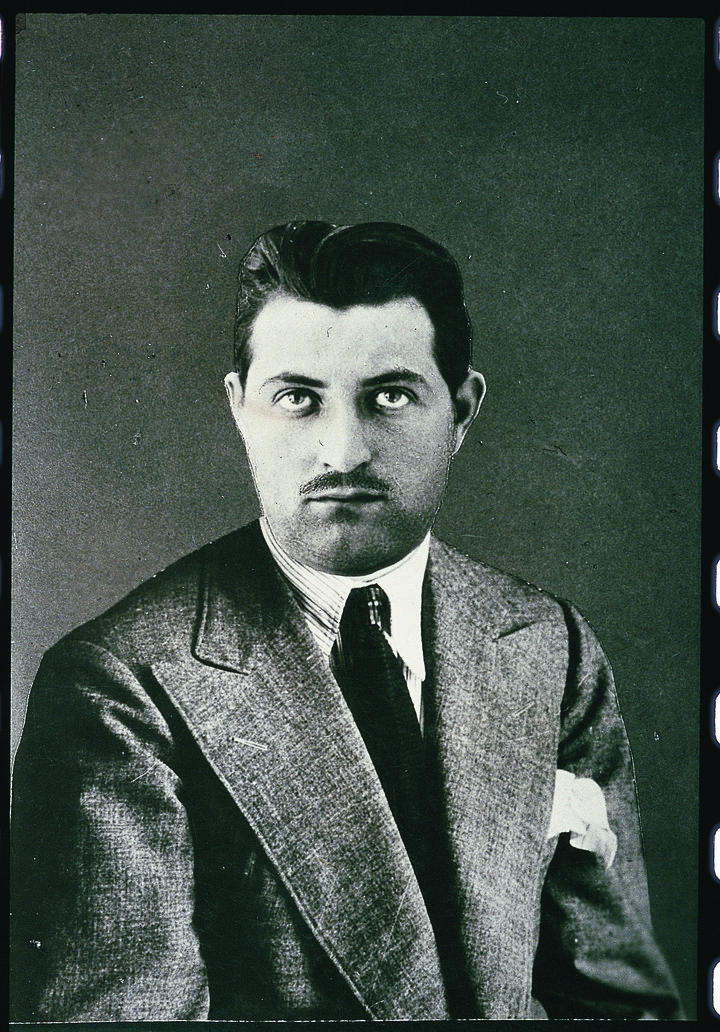
\includegraphics[width=0.5\textwidth]{../Images/SeverinoDiGiovanni.jpg}
 \caption{Severino Di Giovanni, el autor de este apunte. Un anarquista
   libertario, murió luchando por la libertad. Como él, otros miles han muerto
   para que nosotros gocemos de los derechos que tenemos. No te dejes engañar
   por los tristes pregoneros del egoísmo. Amá a tu prójimo y no olvides que si
   sus derechos se vulneran, los tuyos también. Ayudá a tu compañero de estudio,
 defendé tu universidad. }
 \end{figure}

\pagebreak

\tableofcontents
\newpage


\section{P1} 

\textbf{(1)} Un geólogo recoge 10 especímenes de A y 12 de B. 15 son elegidos
al azar. De la función de probabilidad de masa del número de especímenes de tipo
A elegidos.

\small
\begin{quote}

Sea $\Omega$ el espacio muestral, con cada $\omega \in \Omega$ una de las
posibles selecciones de $15$ de entre los $22$ especímenes. Claramente,

\begin{equation*}
  \left| \Omega \right| = \binom{22}{15}
\end{equation*}

Sea $X$ la variable aleatoria para el número de especímenes de tipo $A$ en una
selección aleatoria de $\Omega$. Claramente, para tener $X = k$, con $3 \leq k
\leq 10$, la selección debe ser tal que $k$ muestras sean de tipo $A$ y $15 - k$
muestras sean de tipo $B$. Luego 

\begin{equation*}
  P(X = k) = \frac{\binom{10}{k} \binom{12}{15 - k}}{\binom{22}{15}}
\end{equation*}


\end{quote}
\normalsize


\pagebreak 

\textbf{(2)} Sean $X, Y$ independientes y exponenciales con parámetros $\lambda,
\mu$ respectivamente. Computar $f_{X | Y}(x \mid y)$ y $P(X < Y)$.


\small
\begin{quote}

  $(a)$ Recordemos que $f_{X \mid Y}(x \mid y) = \frac{f_{X, Y}(x,
  y)}{f_Y(y)}$. Como $X, Y$ son independientes, su densidad conjunta es el
  producto de las densidades, y tenemos $f_{X \mid Y}(x \mid y) = (f_X(x)
  f_Y(y))/f_Y(y) = f_X(x)$.

  $(b)$ Veamos que

  \begin{align*}
    P(X < Y) 
    &= \int_{\mathbb{R}} f_Y(y) \int_{-\infty}^y f_X(x) ~ dx ~ dy \\ 
    &=\int_\mathbb{R} \mathcal{I}_{(0, \infty)} \cdot \mu e^{-\mu y}
    \int_{-\infty}^y \mathcal{I}_{(0, \infty)} \lambda e^{-\lambda x} ~ dx ~ dy
    \\ 
    &=\int_0^\infty \mu e^{-\mu y}\int_0^y \lambda e^{-\lambda ~ x}
  \end{align*}

Ahora bien, con $w := -\lambda x, dw = -\lambda dx$, tenemos

\begin{align*}
  \int_0^y \lambda e^{-\lambda x} ~ dx 
  &= -\int_0^{w(y)}  e^w ~ dw \\ 
  &=-\int_0^{-\lambda y} e^w ~ dw \\ 
  &= - \left[ e^{-\lambda y} - e^0 \right] \\ 
  &=1 - e^{- \lambda y}
\end{align*}

Por lo tanto

\begin{align*}
P(X < Y) 
  &= \int_0^\infty \mu e^{-\mu y} \left( 1 - e^{-\lambda ~ y} \right) ~ dy \\ 
  &= \int_0^\infty \mu e^{-\mu y} ~ dy - \int_0^\infty \mu e^{-(\mu + \lambda) y
  } ~ dy \\ 
  &= \int_0^\infty f_{Y}(y) ~ dy - \frac{\mu}{\mu + \lambda}\int_0^\infty (\mu +
  \lambda)e^{-(\mu + \lambda) y} ~ dy \\ 
  &= 1 - \frac{\mu}{\mu + \lambda} \int_0^\infty f_{Z}(y) ~ dy &\left\{ Z \sim
  \mathcal{E}(\mu + \lambda) \right\}  \\ 
  &= 1 - \frac{\mu}{\mu + \lambda} \\ 
  &= \frac{\mu + \lambda}{\mu + \lambda} - \frac{\mu}{\mu + \lambda} \\ 
  &= \frac{\lambda}{\mu + \lambda}
\end{align*}


\end{quote}
\normalsize

\pagebreak

\textbf{(3)} Sean $X, Y$ independientes y exponenciales con el mismo parámetro
$\lambda$. Computar la densidad
condicional de $X$ dado que $X + Y = t$.


\small
\begin{quote}

Por def. de densidad condicional, tomando $T := X + Y$,

  \begin{equation*}
    f_{X \mid T}(x\mid t) = \frac{f_{X, T}(x, t)}{f_T(t)} 
  \end{equation*}

Calculemos estas distribuciones.

\begin{align*}
  f_{X, T}(x, t) 
  &= P(X = x \cap X + Y = t) \\ 
  &= P(X = x \cap Y = t - x) \\ 
  &=P(X = x) \cdot P(Y = t - x) &\left\{ X, Y \text{ son independientes}
  \right\} \\ 
  &= f_X(x) \cdot f_Y(t - x) \\ 
  &= \lambda e^{-\lambda x} \mathcal{I}_{(0, \infty)}(x) \cdot \lambda e^{-\lambda(t - x)} ~ \mathcal{I}_{(0,
  \infty)}(t-x)\\ 
  &= \lambda^2e^{-\lambda t} ~ \mathcal{I}_{(0, \infty)}(t-x) \mathcal{I}_{(0,
  \infty)}(x) \\ 
  &= \lambda^2e^{-\lambda t} ~ \mathcal{I}_{(x, \infty)}(t) \mathcal{I}_{(0,
  \infty)}(x) \\ 
\end{align*}

El último paso se justifica porque $\mathcal{I}_{(0, \infty)}(t-x)\mathcal{I}_{(0,
\infty)}(x) = \mathcal{I}_{(0, \infty)}(x) \mathcal{I}_{(x, \infty)}(t)$. En
efecto, $t - x$ pertenece a $(0, \infty)$ si y solo si $t > x$. Ahora bien,

\begin{align*}
  f_T(t) 
  &= f_{X+Y}(t) \\ 
  &= \int_{\infty}^t f_X(x) f_Y(t - x) ~ dx &\left\{ X, Y \text{ independientes}
  \right\} \\ 
  &= \int_{-\infty}^t \mathcal{I}_{(0, \infty)} \cdot \lambda e^{-\lambda x}
  \cdot \mathcal{I}_{(0, \infty)}(t-x) \lambda
  e^{-\lambda(t - x)} ~ dx \\ 
  &=\int_0^t \lambda^2 e^{-\lambda t} \cdot 
  \mathcal{I}_{(x, \infty)}(t) ~ dx \\ 
  &=\lambda^2 e^{-\lambda  t} \int_0^t \mathcal{I}_{(x, \infty)}(t)~ dx \\ 
  &=\lambda^2 e^{-\lambda  t} \int_0^t 1 ~ dx \qquad (\star)\\ 
  &=t\lambda^2 e^{-\lambda  t} 
\end{align*}

El paso a $(\star)$ se justifica como sigue. Si la región de integración es $(0, t)$ y la variable de
integración es $x$, siempre se cumple que $x < t$, y por lo tanto
$\mathcal{I}_{(x, \infty)}(t) = 1$.

  \begin{equation*}
    \therefore \quad f_{X \mid T}(x\mid t) = \frac{f_{X, T}(x, t)}{f_T(t)} 
    = \frac{\lambda^2 e^{-\lambda t}\mathcal{I}_{(0, \infty)(x)}\mathcal{I}_{(x,
    \infty)}(t)}{t \lambda^2 e^{-\lambda t}} = \begin{cases}
      \frac{1}{t} & 0 \leq x \leq t  \\ 
      0 & c.c.
    \end{cases}
  \end{equation*}

\end{quote}
\normalsize

\pagebreak 

\textbf{(4)} Sean $N_1(t), N_2(t)$ procesos con $t \geq 0$ y tasas $\lambda = 1,
\mu = 2$ respectivamente. Sea $N(t) = N_1(t) + N_2(t)$. 

$(a)$ Calcular la probabilidad de que $N(1) = 2, N(2) = 5$.

$(b)$ Calcular la probabilidad de que $N_1(1) = 1$ dado $N(1) = 2$.

$(c)$ Calcular la probabilidad de que el segundo arribo en $N_1$ ocurra antes
que el tercer arribo en $N_2(t)$.


\small
\begin{quote}

$(a)$ Es muy fácil porque $N(t)$ es un proceso de Poisson con parámetro $\lambda
+ \mu = 3$, con lo cual $P(N(t) = k) = e^{-3} \frac{3^k}{k!}$ para cualquier $k
\geq 0$ entero.

~ 

$(b)$ Claramente, si $N(1) = 2$, la probabilidad de que $N_1(1) = 1$ es la
probabilidad de que $N_2(1) = 1$.

\begin{align*}
  P(N_1(1) = 1 \mid N(1) = 2) 
  &= \frac{P(N_1(1) = 1 \cap N(1) = 2)}{P( N(1) = 2 )} \\ 
  &= \frac{ P(N_1(1) = 1 \cap  N_1(1) + N_2(1) = 2) }{P(N(1) = 2)} \\ 
  &= \frac{ P(N_1(1) = 1 \cap N_2(1) = 1) }{P(N(1) = 2)} \\ 
  &=\frac{ P(N_1(1) = 1) \cdot P(N_2(1) = 1) }{P(N(1) = 2)} &\left\{
  \text{Independencia de } N_1, N_2 \right\} 
\end{align*}

Ahora solo resta ver que 

\begin{equation*}
  e^{-\lambda ~ l} \frac{( \lambda l)^k}{k!} \leq e^{- \mu ~ l} \frac{( \mu l )^k}{k!} \iff
  e^{-\lambda l} \lambda^k \leq e^{-\lambda \mu} \mu^k \iff \lambda  \ln
  \lambda \geq \mu  \ln \mu
\end{equation*}

\begin{align*}
  P(N_1(1) = 1) &= e^{-1} \frac{1^1}{1!} = e^{-1} \approx 0.368 \\ 
  P(N_2(1) = 1)&= e^{-2} \frac{2^1}{1!} = 2e^{-2} \approx 0.27\\ 
  P(N(1) = 2) &= e^{-3} \frac{3^2}{2!} = \frac{9}{2}e^{-3} \approx 0.224
\end{align*}

\begin{equation*}
  \therefore P(N_1(1) = 1 \mid N(1) = 2) \approx \frac{0.368 \cdot 0.27}{0.224}
  = 0.443
\end{equation*}

Otra forma de calcularlo es usando el teorema de Bayes:

\begin{align*}
  P(N_1(1) = 1 \mid N(1) = 2) 
  &= \frac{P(N(1) = 1 \mid N_1(1) = 1) P(N_1(1) =
  1)}{P(N(1) = 1)} \\ 
  &= \frac{P(N_1(1) + N_2(1) = 1 \mid N_1(1) = 1) P(N_1(1) = 1)}{P(N(1) = 1)} \\ 
  &=\frac{ P(N_2(1) = 1) \cdot P(N_1(1) = 1) }{P(N(1) = 2)}
\end{align*}

que es lo mismo que tuvimos antes.

$(c)$ Se nos pide la probabilidad de que el segundo arribo en $N_1(t)$ ocurra antes
que el tercer arribo en $N_2(t)$. A primera vista no parece, pero este es
simplemente un problema de conteo. 

Primero, observemos que el evento "el segundo arribo en $N_1(t)$ ocurre antes
que el tercero de $N_2(t)$" es equivalente al evento "de $4$ eventos en $N(t)$,
al menos dos provienen de $N_1(t)$". Sea $\omega$ este evento.

La probabilidad de que un evento dado de $N(t)$ provenga de $N_1(t)$ es
$\frac{\lambda}{\lambda + \mu}$. La probabilidad de que un evento dado de $N(t)$
provenga de $N_2(t)$ es $\frac{\mu}{\lambda + \mu}$.

\begin{align*}
  \therefore ~ P(\omega) 
  &= \binom{4}{2} \frac{\lambda^2\mu^2}{( \lambda + \mu
  )^4} + \binom{4}{3} \frac{\lambda^3 \mu}{(\lambda + \mu)^4} +
  \binom{4}{4}\frac{\lambda^4}{(\lambda+ \mu)^4}
\end{align*}

Sustituyendo $\lambda, \mu$ por sus valores y calculando los binomiales, que son
fáciles, sale el resultado.


\end{quote}
\normalsize

\pagebreak 

\textbf{(5)} Sean $X, Y$ independientes con distribuciones de Poisson
parametrizadas bajo $\lambda, \mu$ respectivamente. Probar que 
$Z = X + Y \sim \mathcal{P}(\lambda + \mu)$.


\small
\begin{quote}

Como son independientes, la distribución de su suma es dada por la "convolución"
discreta de sus distribuciones. Si con $\mathbb{N}$ denotamos los naturales y
el cero, entonces

\begin{align*}
  f_{Z}(z)  
  &=\sum_{k \in \mathbb{N} } p_X(k) p_Y(z - k)  \\ 
  &=\sum_{k \in \mathbb{N}} \left( e^{-\lambda} \frac{\lambda^k}{k!} \right)
  \left( e^{- \mu} \frac{\mu^{z - k}}{(z-k)!} \right)  \\ 
  &=e^{-\lambda }e^{-\mu} \sum_{k \in \mathbb{N}} \frac{\lambda^k
  \mu^{z-k}}{k!(z-k)!} \\ 
  &= \frac{\eta}{z!} \sum_{k \in \mathbb{N}} \lambda^k \mu^{z-k}\frac{z!}{k!(z -
k)!} &\left\{ \eta := e^{-\lambda }e^{-\mu} \right\}  \\ 
     &= \frac{\eta}{z!} \sum_{k\in \mathbb{N}} \lambda^k \mu^{z-k} \binom{z}{k}
\end{align*}

Ahora bien, como $Y \sim \mathcal{P}(\mu)$, $Im(Y) = \mathbb{N}$, y por lo tanto
$p_Y(u) = 0$ si $u < 0$. En otras palabras, dado un $k$ arbitrario, 
$p_Y(z - k) \neq 0 \iff z - k \geq 0 \iff k \leq z$.

\begin{equation*}
  &\therefore \frac{\eta}{z!} \sum_{k\in \mathbb{N}} \lambda^k \mu^{z-k}
  \binom{z}{k} 
  = \frac{\eta}{z} \sum_{k = 0}^z \lambda^k \mu^{z-k}\binom{z}{k} =
  \frac{\eta}{z!} (\lambda + \mu)^z = e^{-(\lambda + \mu)}\frac{(\lambda+\mu)^z}{z!}
\end{equation*}

por el teorema del binomio de Newton. 

$\therefore $ $Z \sim \mathcal{P}(\lambda + \mu)$. $\qquad \blacksquare$

\end{quote}
\normalsize

\pagebreak 

\section{P3}


\textbf{(2)} (Todas las variables en este problema son uniformes continuas e
independientes en
$(0, 1)$).
En un juego, se simula la variable aleatoria $U$.
Si $U < \frac{1}{2}$ se suman dos números aleatorios. Si $U \geq
\frac{1}{2}$, se suman tres. El resultado $X$ de cualquiera de estas sumas
es el puntaje, y se tiene éxito si $X \geq 1$.

~

$(a)$ Dar la probabilidad de ganar.


\small
\begin{quote}

Por ley de probabilidad total,

\begin{align*}
  &P(X_1 + X_2 \geq 1 \mid U < \frac{1}{2})P(U < \frac{1}{2}) + P(X_1 +
  X_2 + X_3 \geq 1\mid
  U \geq \frac{1}{2})P(U \geq \frac{1}{2}) \\ 
  =&P(X_1 + X_2 \geq 1)P(U < \frac{1}{2}) + P(X_1 + X_2 + X_3 \geq 1)P(U \geq
  \frac{1}{2})\\
  =&P(X_1 + X_2 \geq 1)\cdot \frac{1}{2} + P(X_1 + X_2 + X_3 \geq
  1)\cdot \frac{1}{2}
\end{align*}

Estudiemos $P(X_1 + X_2 = z)$. Veamos que si $z \in [0, 1]$, entonces

\begin{equation*}
  P(X_1 + X_2 = z) = \int_0^z f_{X_1}(x)f_{X_2}(z-x) ~ dx = \int_0^z 1 ~ dx 
  =z
\end{equation*}

Si $z \in (1, 2]$, entonces hacemos variar $X_1$ entre $[z-1, 1]$ y requerimos
$X_2 = z - X_1$:

\begin{equation*}
  P(X_1 + X_2 = z) 
  = \int_{z-1}^{1} f_{X_1}(x) f_{X_2}(z - x) ~  dx = 2 -z
\end{equation*}



\begin{equation*}
  \therefore ~ f_{X_1 + X_2}(x) = \begin{cases}
    x & 0 \leq x \leq 1 \\ 
    2 - x & 1 < x \leq 2 \\ 
    0 & c.c.
  \end{cases}
\end{equation*}

Por lo tanto,

\begin{equation*}
  P(X_1 + X_2 \geq 1) = \int_1^2 f_{X_1 + X_2}(x) ~ dx = \int_1^2(2-x) ~ dx =
  1 / 2
\end{equation*}

Resta ver que 

\begin{align*}
  P(X_1 + X_2 + X_3 \geq 1) 
  &= P(X_1 + X_2 \geq 1 - X_3) \\ 
  &=\int_0^1  P(X_1 + X_2 \geq 1 - z) P(X_3 = z) ~ dz &\left\{ \text{Por prob.
  total} \right\} \\ 
  &=\int_0^1 \left(1 - \frac{(1-z)^2}{2}\right) \cdot 1 ~ dz &\left\{ \text{Por }
  \star\right\} \\ 
  &=5 / 6
\end{align*}

dado que para $z \in [0, 1]$

\begin{equation*}
  ( \star ) \qquad P(X_1 + X_2 \geq 1 - z) = 1 - P(X_1 + X_1 \leq 1 - z) = 1 - \int_0^{1-z} x ~ dx = 1 - \frac{ (1-z)^2 }{2}
\end{equation*}

\begin{align*}
  \therefore  ~ ~ ~
  &P(X_1 + X_2 \geq 1)\cdot \frac{1}{2} + P(X_1 + X_2 + X_3 \geq
  1)\cdot \frac{1}{2} \\
  = &\frac{1}{2} \cdot \frac{1}{2} + \frac{5}{6} \cdot
  \frac{1}{2}  \\
  = &\frac{1}{4} + \frac{5}{12} \\
  =&\frac{2}{3}
\end{align*}

\end{quote}
\normalsize


~

$(b)$ Implement an algorithm that estimates the probability of winning, i.e. the
proportion of wins in $n$ simulations of the game.

~ 

In Python, 




\tiny
\begin{quote}

\begin{verbatim}[python]
from random import uniform

def sim_2(n):

  wins = 0

  # S = summation of uniform rvs
  def S(k):
    return sum( [uniform(0, 1) for _ in range(k)] )

  for _ in range(n):

    u = uniform(0, 1)
 
    X = S(2) if u < 0.5 else S(3)
    wins = wins + 1 if X >= 1 else wins

  return wins/n
\end{verbatim}




\end{quote}
\normalsize
\pagebreak 

\textbf{(3)} Las máquinas tragamonedas usualmente generan un premio cuando hay un acierto. Supongamos que se genera el acierto con el siguiente esquema: se genera un número aleatorio, y

\begin{itemize}
\item si es menor a un tercio, se suman dos nuevos números aleatorios
\item si es mayor o igual a un tercio, se suman tres números aleatorios .
\end{itemize}

Si el resultado de la suma es menor o igual a 2, se genera un acierto.

~

$a)$ ¿Cuál es la probabilidad de acertar?.


\small
\begin{quote}

Sea $Z_n = \sum_{i=1}^n U_i$ con $U_i \sim \mathcal{U}(0, 1)$ para $1 \leq i
\leq n$. Por ley de probabilidad total, se llega con facilidad a

\begin{equation*}
  P(\text{Ganar}) = P(Z_2 \leq 2) \cdot \frac{1}{3} + P(Z_3 \leq 2) \cdot
  \frac{2}{3}
\end{equation*}

Claramente, $P(Z_2 \leq 2) = 1$, con lo cual solo queda computar $P(Z_3 \leq
2) = P(Z_2 \leq 2 - U_3)$. La densidad de $Z_2$ fue calculada en el punto
$\textbf{(2)}$. Para calcular $P(Z_3 \leq 2)$, podemos hacer variar a $U_3$ en
todo el rango $[0, 1]$ y a $Z_2$ en todo el rango $[ 0, 2 - U_3 ]$:

\begin{align*}
  P(Z_3 \leq Z_2) 
  &= P(Z_2 \leq 2 - U_3) \\ 
  &=\int_0^1 P(U_3 = z) \int_{0}^{2-z} f_{Z_2}(x) ~ dx ~ dz \\ 
  &=\int_0^1 \left[ \int_0^1 f_{Z_2}(x) ~ dx + \int_1^{2 - z} f_{Z_2}(x) ~ dx
  \right] ~ dz \\ 
  &=\int_0^1 \left[ \int_0^1 x ~ dx + \int_1^{2-x}(2-x) ~ dx  \right] ~ dz \\ 
  &= \int_0^1 \left[ \frac{1}{2} - \frac{z^2}{2} + \frac{1}{2}\right]  ~ dz \\ 
  &=\int_0^1 1 - \frac{z^2}{2} ~ dz \\ 
  &= 5 / 6
\end{align*}


Una forma alternativa de calcular esta probabilidad es hacer variar a $Z_2$ en
todo el rango $[0, 2]$ y luego hacer variar a $U_3$ en todo el rango $[0, 2 -
Z_2]$:

\begin{align*}
  P(Z_3 \leq 2) 
  &=P(Z_2 \leq 2 - U_3)\\
  &= \int_0^2 f_{Z_2}(x) \int_0^{2-x} f_{U_3}(y) ~ dy ~ dx \\ 
  &= \int_0^1 f_{Z_2}(x) \int_0^{1} f_{U_3}(y) ~ dy ~ dx + \int_1^2 f_{Z_2}(x)
  \int_0^{2-x} f_{U_3}(y) ~ dy ~ dx &\left\{ \text{Por } \star \right\}  \\
                                    &=\int_0^1 x \int_0^1 1 ~ dy ~ dx +
                                    \int_{1}^2 (2-x) \int_0^{2 - x} 1 ~ dy ~ dx\\
  &=\int_0^1 x ~ dx + \int_1^2 (2-x)^2 ~ dx \\
  &=\frac{1}{2} + \frac{1}{3} \\ 
  &= \frac{5}{6}
\end{align*}

\begin{quote}
  ($\star$) Si $Z_2$ varía en $[0, 1]$, $Z \leq 2 - U_3$ para cualquier valor de
  $U_3$, con lo cual hacemos a $U_3$ variar en todo el rango $[0, 1]$.  Pero si
  $Z_2$ varía en $[1, 2]$, entonces $U_3$ solo puede tomar valores en $[0, 2 -
  Z_2]$.
\end{quote}

\begin{align*}
  \therefore \qquad P(\text{Ganar}) 
  &= P(Z_2 \leq 2) \cdot \frac{1}{3} + P(Z_3 \leq 2) \cdot
  \frac{2}{3} \\ 
  &= \frac{1}{3} + \frac{5}{6}\frac{2}{3} \\ 
  &= 0.\overline{8}
\end{align*}

\end{quote}
\normalsize



$b)$ Implementar un algoritmo en computadora que estime la probabilidad de acertar, esto es, la fracción
de veces que se acierta en $n$ realizaciones del juego. 

En Python, una implementación posible es:

\small
\begin{quote}

\begin{verbatim}
from random import uniform

def sim_3(n):
  wins = 0 

  # S = summation of uniform r.vs
  def S(k): 
    return sum( [uniform(0, 1) for _ in range(k)] )

  for _ in range(n):
    u = uniform(0, 1)
    X = S(2) if u < 1/3 else S(3)
    wins = wins + 1 if X <= 2 else wins

  return wins/n
\end{verbatim}

\end{quote}
\normalsize

\pagebreak 

(\textbf{4}) Un supermercado posee 3 cajas. Por una cuestión de ubicación, el
40\% de los clientes eligen la caja 1 para pagar, el 32\% la caja 2, y el 28\%
la caja 3. 

El tiempo que espera una persona para ser atendida en cada caja
distribuye exponencial con medias de 3, 4 y 5 minutos respectivamente. 

~

$(a)$ ¿Cuál es la probabilidad de que un cliente espere menos de 4 minutos para ser
atendido? 


\small
\begin{quote}

Recordemos que la media de la exponencial es $1 / \lambda$, es decir que
$\lambda_1 = 1 / 3, \lambda_2 = 1 / 4, \lambda_3 = 1 / 5$.

El evento "un cliente espera menos de $4$ minutos en ser atendido" se divide en
un sub-eventos correspondiente por cada caja. Más formalmente, si $T$ es el
tiempo de espera de un cliente arbitrario, y $C_i$ el evento de que el cliente
elige la i-ésima caja, entonces por ley de probabilidad total:

\begin{equation*}
  P(T \leq 4) = \sum_{i=1}^3 P(C_i)P(T \leq 4 \mid C_i) = \sum_{i=1}^3 P(C_i)
  P(X_i \leq 4)
\end{equation*}

donde $X_i$ es una exponencial con parámetro $\lambda_i$. En general, 

\begin{equation*}
  \int_0^4 \lambda_i e^{-\lambda_i x} ~dx = 1 - e^{-4\lambda_i}
\end{equation*}

de lo cual se sigue: 

\begin{equation*}
  P(X_i \leq 4) = \begin{cases}
    0.736 & i = 1 \\ 
    0.632 & i = 2\\ 
    0.55 & i = 3
  \end{cases}
\end{equation*}

\begin{equation*}
  \therefore P(T\leq 4) = 0.40 \cdot 0.736 + 0.32 \cdot 0.632 + 0.28 \cdot 0.55
  = 0.65064
\end{equation*}


\end{quote}
\normalsize


~

$(b)$ Si el cliente tuvo que esperar más de 4 minutos. ¿Cuál es la
probabilidad de que el cliente haya elegido cada una de las cajas? 


\small
\begin{quote}

  Sale fácil con teorema de Bayes y los resultados de $(a)$:

  \begin{equation*}
    P(C_i \mid T \leq 4) 
    &= \frac{P(T \leq 4 \mid C_i)P(C_i)}{P(T \leq 4)}
  \end{equation*}

\end{quote}
\normalsize


~

$(c)$ Simule el
problema y estime las probabilidades anteriores con 1000 iteraciones.

An ugly Python implementation:


\small
\begin{quote}

\begin{verbatim}
from numpy.random import exponential
from random import uniform

def sim_4(n):

  wins = 0
  rates = [1/3, 1/4, 1/5]

  def choose_rate(x):
    if x <= 0.4:
      return 0 
    return 1 if u <= 0.4 + 0.32 else 2

  for _ in range(n): 

    u = uniform(0, 1)
    rate = rates[choose_rate(u)]

    e = exponential(1/rate)

    wins = wins + 1 if e <= 4 else wins

  return wins/n 


\end{verbatim}

\end{quote}
\normalsize

\pagebreak 

\textbf{(5)} Calcule con el método de Monte Carlo y escriba simulaciones para
cada una de las siguientes integrales. 

~ 

$(a)$ $\int_0^1 (1-x^2)^{3 / 2} ~ dx$


\small
\begin{quote}

Sea $f_U(x)$ la densidad de $U \sim \mathcal{U}(0, 1)$. Entonces 

\begin{equation*}
  \theta := \int_0^1(1-x^2)^{3 / 2} ~ dx = \int_0^1 (1-x^2)^{3 / 2} f_U(x) ~ dx =
  \mathbb{E}\left[ g(U) \right] 
\end{equation*}

con $g(x) = (1-x^2)^{3 / 2}$. Por lo tanto, $\theta \approx \frac{1}{n}
\sum_{i=1}^n g(u_i)$ con $u_1, \ldots, u_n$ realizaciones de $U_1, \ldots, U_n
\sim \mathcal{U}(0, 1)$. Es decir, 

\begin{equation*}
  \theta \approx \frac{1}{n} \sum^n (1 - u_i^2)^{3 / 2}
\end{equation*}

En Python,

\begin{quote}
\begin{verbatim}
from random import uniform
def sim_5a(n):
  uniforms = [uniform(0, 1) for _ in range(n)]
  return 1/n * sum( [ (1 - u**2)**1.5  for u in uniforms ] )

\end{verbatim}
\end{quote}

\pagebreak

\end{quote}
\normalsize

$(b) \int_2^3 \frac{x}{x^2-1} ~ dx$


\small
\begin{quote}

Si hacemos $u = x - 2$, tal que $du = dx$ y $x = 2 + u$, tenemos 

\begin{equation*}
  \theta := \int_2^3 \frac{x}{x^2 - 1} ~ dx = \int_0^1 \frac{2+u}{(2+u)^2 - 1} ~ du =
  \int_0^1 \frac{2+u}{u^2 - 4u + 3}
\end{equation*}

Entonces $\theta = \int_0^1 g(x)f_U(x) ~ dx = \mathbb{E}\left[ g(U) \right] $
con $U \sim \mathcal{U}(0, 1), g(x) = \frac{2+x}{(2+x)^2 - 1}$. 

\begin{equation*}
  \therefore ~ \theta \approx \frac{1}{n}\sum_{i=1}^n \frac{2 + u_i}{u_i^2
  -4u_i + 3}
\end{equation*}

donde $u_1, \ldots, u_n$ son realizaciones de $U_1, \ldots, U_n \sim
\mathcal{U}(0, 1)$ independientes para $n \geq 1$. En Python, 

\footnotesize
\begin{quote}
  
\begin{verbatim}
def sim_5b(n):
  uniforms = [uniform(0, 1) for _ in range(n)]
  return 1/n * sum( [ (2 + u)/((2+u)**2 - 1) for u in uniforms ] )
\end{verbatim}
\end{quote}
\small

Con $n = 1000$ obtuve $\theta \approx 0.487$, y el valor real de la integral es $\theta = 0.49$.

\end{quote}
\normalsize
\pagebreak

$(c) \int_0^\infty x(1+x^2)^{-2} ~ dx$


\small
\begin{quote}

Sea $u := \frac{1}{x + 1}$, de manera que 

\begin{equation*}
  du = -\frac{1}{(x+1)^2} ~ dx = -u^2 ~ dx, \qquad x = \frac{1-u}{u} =
  \frac{1}{u} - 1
\end{equation*}

Entonces 

\begin{align*}
  \theta := \int_0^\infty g(x) ~ dx = -\int_0^1 \frac{g(\frac{1}{u} - 1)}{u^2}
  ~ du = -\int_0^1 \frac{(\frac{1}{u} - 1)(1 + (\frac{1}{u} - 1)^2)^{-2}}{u^2} ~
  du
\end{align*}

Luego 

\begin{equation*}
  \theta = -\int_0^1 \psi(u) f_U(u) ~ du = -\mathbb{E}\left[ \psi(U) \right] 
\end{equation*}

con $\psi(u) = g(\frac{1}{u} - 1) / u^2$ y $U \sim \mathcal{U}(0, 1)$. En
consecuencia, 

\begin{equation*}
  \theta \approx \frac{1}{n}\sum_{i=1}^n \psi(u_i)
\end{equation*}

donde $u_1, \ldots, u_n$ son realizaciones de $U_1, \ldots, U_n \sim
\mathcal{U}(0, 1)$ independientes (no confundir con $u$, la variable de
integración) y $n \geq 1$. En Python, 

\footnotesize 

\begin{verbatim}
def sim_5c(n):
  uniforms = [uniform(0, 1) for _ in range(n)]

  def h(u):
    return (1/u - 1)*(1 + (1/u - 1)**2)**(-2) * (1/u**2)

  return 1/n * sum( [h(u) for u in uniforms] )
\end{verbatim}

\small 

Con $n = 1000$, la simulación dio $\varphi \approx 0.504$, y el valor real de la
integral es $\theta = \frac{1}{2}$.


\end{quote}
\normalsize

\pagebreak
\pagebreak

$(d) \int_{-\infty}^\infty e^{-x^2} ~ dx$


\small
\begin{quote}

Let $g(x) := e^{-x^2}$. Clearly, $g(-x) = e^{-(-x^2)} = g(x)$, which means $g$
is symmetric.

$\therefore ~ \int_{-\infty}^\infty e^{-x^2} ~ dx = 2\int_0^\infty e^{-x^2} ~
dx$. If we let 

\begin{equation*}
  \psi = \frac{1}{x+1}, \qquad d \psi = -\psi^2, \qquad x = \frac{1}{\psi}-1
\end{equation*}

Entonces

\begin{equation*}
  \theta := 2\int_0^\infty e^{-x^2} = 2\int_0^1 \frac{\exp\left(-\left(\left(\frac{1}{\psi} -
  1\right)^2\right)\right)}{\psi^2} f_U(\psi) ~ d\psi
\end{equation*}

donde $f_U$ es la densidad de $U \sim \mathcal{U}(0, 1)$. $\therefore
\theta = \mathbb{E}\left[ h(U) \right] $ con $h(x) =
\exp\left(-\left(\left(\frac{1}{x}-1\right)^2\right) /
x^2$. 

\begin{equation*}
  \therefore \quad \theta \approx \frac{1}{n}\sum_{i=1}^n 
  \frac{\exp\left(-\left(\left(\frac{1}{u_i} - 1\right)^2\right)\right)}{u_i^2}, \qquad n \geq 1
\end{equation*}

con $u_1, \ldots, u_n$ realizaciones de $U_1, \ldots, U_n \sim \mathcal{U}(0,
1)$. En Python,

\footnotesize 

\begin{verbatim}
from math import exp 
from random import uniform
  
def sim_5d(n):
    def h(u):
        return exp(-(( 1/u - 1 )**2)) / (u**2)

    uniforms = [uniform(0, 1) for _ in range(n)]
    return 2*sum([ h(u) for u in uniforms ]) / n
\end{verbatim}

\small 

La simulación con $n = 1000$ dio $\theta \approx 1.73$ que es casi exactamente
$\sqrt{\pi}$, el verdadero valor.

\textbf{Nota.} El ejercicio se puede resolver aplicando directamente la
sustitución sin notar que $g$ es simétrica, aunque se dan pasos previos algo más
engorrosos:

\begin{align*}
  \int_{-\infty}^\infty g(x) ~ dx 
  &= \lim_{t \to -\infty}\int_t^0 g(x) ~dx +
  \lim_{t \to \infty} \int_0^\infty g(x) ~ dx \\ 
  &=-\int_{\lim_{t \to -\infty} \psi(t)}^0 \frac{ g(\frac{1}{\psi} - 1) }{\psi^2}
  ~ d\psi - \int_0^{ \lim_{t \to \infty} \psi(t)} 
  \frac{g(\frac{1}{\psi} - 1)}{\psi^2} ~ d\psi \\ 
  &=\int_0^1 \frac{g(\frac{1}{\psi} - 1)}{\psi^2} ~ d\psi + \int_0^1
  \frac{g(\frac{1}{\psi} - 1)}{\psi^2} ~ d\psi \\ 
  &= 2 \int_0^1 \frac{g(\frac{1}{\psi} - 1)}{\psi^2} ~ d\psi
\end{align*}

A partir de acá todo es igual.


\end{quote}
\normalsize

\pagebreak
$(e)$ $\theta := \int_0^1 \int_0^1 \exp(( x+y )^2) ~ dx ~ dy$


\small
\begin{quote}

Let $X, Y \sim \mathcal{U}(0, 1)$ independent with densities $f_Y, f_U$. Clearly, their
joint density function is 

\begin{equation*}
  f_{X, Y}(x, y) = f_X(x)f_Y(y) = \mathcal{I}_{(0, 1) \times (0, 1)}
\end{equation*}

Then 

\begin{equation*}
  \theta = \int_0^1 \int_0^1 g(x, y) f_{X, Y}(x, y) ~ dx ~ dy = \mathbb{E}\left[
  g(X, Y)\right] 
\end{equation*}

\begin{equation*}
  \therefore \quad \theta \approx \frac{1}{n} \sum_{i=1}^{n} g(x_i, y_i), \qquad
  n \geq 1
\end{equation*}

where $(x_1, y_1), \ldots, (x_n,y_n)$ are realizations of $(X_1, Y_1),
\ldots, (X_n, Y_n)$, with $X_i, Y_i \sim \mathcal{U}(0, 1)$ for $1 \leq i \leq
n$.

In Python,

\footnotesize 

\begin{verbatim}
from math import exp 
from random import uniform 

def sim_5e(n):
    def g(x, y):
        return exp((x+y)**2)
    
    X = [uniform(0, 1) for _ in range(n)]
    Y = [uniform(0, 1) for _ in range(n)]

    return sum([ g(x, y) for x, y in zip(X, Y) ]) / n
\end{verbatim}

With $n = 100000$, the estimation was $4.902$, and the true value of the
integral according to Wolfram Alpha is $4.899$.

\end{quote}
\normalsize


\pagebreak 

\textbf{(7)} Definamos 

\begin{equation*}
  N = \min_{n} \left\{ n : \sum_{i=1}^n U_i > 1 \right\}, \qquad U_i \sim
  \mathcal{U}(0, 1)
\end{equation*}

$(a)$ Estimar $\mathbb{E}[N]$ generating $n$ values for $N$.

$(b)$ Calculate $E[N]$.


\small
\begin{quote}

Notemos que $Im(N) = \left\{ 2, 3, \ldots \right\} $. Calculemos $p_N(n)$ la
función de probabilidad de masa de $N$. Para ello, observemos que 

\begin{equation*}
  P(N = n) = P\left(\sum_{i=1}^{n-1} U_i \leq 1 \cap U_n > 1 - \sum_{i=1}^{n-1}
  U_i\right)
\end{equation*}

Sea $X(n) = \sum_{i=1}^n U_i$ y, para simplificar la notación, usemos
$\varphi(n, x) := P(X(n) \leq x)$ para $x \geq 0$. Es decir, $\varphi(n, x)$ es
la función de probabilidad acumulada de $X(n)$. Entonces, la expresión de arriba
nos queda

\begin{equation*}
  P(N = n) = P(X(n-1) < 1 \cap U_n > 1 -X(n-1)) 
\end{equation*}

De acuerdo con la ley de probabilidad total,


\begin{align*}
  \varphi(n, x) 
  &= P(X(n) \leq x) \\
  &= P(U_n \leq x - X(n-1)) \\
  &= \int_{\mathbb{R}} P(U_n \leq x-z) P\left( X(n-1) = z \right) ~ dz \\ 
  &=\int_0^{x} (x-z) \frac{d}{dz} \varphi(n-1, z) ~ dz
\end{align*}

donde estamos utilizando el hecho de que la función de densidad es la derivada
de la función de probabilidad acumulada. Esta expresión recursiva de $\varphi(n, x)$
nos permite avanzar: si restringimos $x \in [0, 1]$,


\begin{align*}
  \varphi(2, x) 
  &= \int_0^x(x-z)\frac{d}{dz}\varphi(1, z) ~ dz \\
  &=\int_0^x(x-z) ~ dz \\ 
  &= \frac{x^2}{2}
\end{align*}

Siguiendo probando casos, obtenemos

\begin{align*}
  f(x, 3) &= \int_0^x(x-z)z ~ dz = \frac{x^3}{6} \\
  f(x, 4) &= \int_0^x(x-z)\frac{z^2}{2} ~ dz = \frac{x^4}{24} \\
          &\vdots \\ 
  f(x, n) &= (x-t) \frac{d}{dz}\varphi(x, n-1)(x:=z) ~ dz = \frac{x^n}{n!}
\end{align*}

Es decir, obtenemos una expresión general para la probabilidad acumulada de
$X(n)$, de lo cual se deduce que la densidad de $X(n)$ es 

\begin{equation*}
  \psi(n, x) = \frac{d}{dx} \frac{x^n}{n!} = \frac{nx^{n-1}}{n!} =
  \frac{x^{n-1}}{(n-1)!} = \varphi(n-1, x), \qquad 0 \leq x \leq 1
\end{equation*}

Por lo tanto,

\begin{align*}
  P(N = n) 
  &= P(X(n-1) < 1 \cap U_n > 1 -X(n-1)) \\ 
  &=\int_0^1 \psi(n-1, x) P(U_n > 1 - x) ~ dx \\ 
  &=\int_0^1 \frac{x^{n-2}}{(n-2)!}(1 - P(U_n \leq 1-x)) ~ dx \\ 
  &=\frac{1}{(n-2)!}\int_0^1  x^{n-1} ~ dx \\ 
  &=\frac{1}{(n-2)!} \frac{1^n}{n} \\ 
  &= \frac{1}{n(n-2)!}
\end{align*}

Por lo tanto, 

\begin{equation*}
  \mathbb{E}\left[ N \right] = \sum_{i=2}^\infty \frac{1}{(n-2)!} =
  \sum_{i=0}^\infty \frac{1}{n!} = e
\end{equation*}

La simulación está de acuerdo, porque en Python 

\begin{verbatim}
def sim_7(iterations):

  counts = []
  n, s = 0, 0

  for _ in range(iterations):
    while s <= 1:
      n += 1
      s += uniform(0, 1)
    counts.append(n)
    n, s = 0, 0
 
  return sum(counts)/len(counts)
\end{verbatim}

nos devuelve siempre aproximadamente $e$.

\pagebreak 

$\textbf{(8)}$ Sea  

\begin{equation*}
  N = \max_{n} \left( \prod_{i=1}^n U_i \geq e^{-3} \right) 
\end{equation*}

con $\prod_{i=1}^0 U_i = 1$. Estimar mediante simulaciones $E[N]$ y $P(N = n)$
para $0 \leq n \leq 6$.

~

\textbf{Solución.} Estimar con simulaciones es aburrido y fácil. Más vale pensemos en el problema y
tratemos de dar $p_N$, la función de probabilidad de masa de $N$.

Claramente, 

\begin{align*}
  P(N = n) 
  &= P \left( \prod_{i=1}^{n-1} U_i \geq e^{-3} \cap U_n \cdot \prod_{i=1}^{n-1}
  U_i < e^{-3}\right) \\ 
  &= P \left( \prod_{i=1}^{n-1} U_i \geq e^{-3} \cap U_n  <
    \frac{e^{-3}}{\prod_{i=1}^{n-1}U_i < e^{-3}}\right) 
\end{align*}

Para simplificar la notación, hagamos $X(n) := \prod_{i=1}^n U_i$ y $\varphi(n,
x) = P(X(n) \leq x)$ para $x \in [0, 1]$. Es decir, $\varphi$ es la CDF de
$X(n)$. Asumimos que $X(0) = 1$, con lo cual $\varphi(0, x) = 1$. Es fácil ver
que $\varphi(1, x) = x$. Veamos además que 

\begin{align*}
  \varphi(2, x) 
  &= P(U_1 U_2 \leq x) \\ 
  &= P(U_1 \leq \frac{x}{U_2}) \\ 
  &= \int_0^1 P(U_1 \leq \frac{x}{z}) P(U_2 = z) ~ dz  \\ 
  &= \int_0^1 P\left( U_1 \leq \frac{x}{z} \right)  ~ dz
\end{align*}

Como $x / z \leq 1$ para $z \in [x, 1]$ y $x / z > 1$ para $z \in [0, x)$,

\begin{align*}
  \int_0^1 P\left( U_1 \leq \frac{x}{z} \right) ~ dz 
  &=\int_0^x P\left( U_1 \leq \frac{x}{z} \right) ~ dz + \int_x^1 P\left( U_1
  \leq \frac{x}{z} \right) ~ dz \\ 
  &= \int_0^x 1 ~ dz + \int_x^1 \frac{x}{z} ~ dz \\ 
  &= x + x \Big[ \ln z\Big]_x^1 \\ 
  &= x - x \ln x
\end{align*}

\begin{myframe}
  Una forma alternativa de dar con la probabilidad buscada es la siguiente:
  
\begin{align*}
  \varphi(2, x) 
  &= P(U_1 U_2 \leq x)  \\ 
  &=\int_0^x \int_0^1 ~ dy ~ dz + \int_x^1 \int_{0}^{x / z} ~ dy ~ dz \\ 
  &=\int_0^x ~ dz + \int_{x}^1 \frac{x}{z} ~ dz \\ 
  &= x + x \int_x^1 \frac{1}{z} ~ dz \\ 
  &= x + x \Big[ \ln z \Big]_{x}^1 \\ 
  &= x + x(\ln 1 - \ln x) \\ 
  &= x - x \ln x
\end{align*}

La forma dada antes, usando la ley de probabilidad total, es más complicada para
este caso particular, pero más útil para el caso general.
\end{myframe}

Generalizando, llegamos a

\begin{align*}
  \varphi(n, x) 
  &= P\left(\prod_{i=1}^{n-1} U_i \leq \frac{x}{U_n}\right)  \\ 
  &= \int_0^1 \varphi\left(n-1, \frac{x}{z}\right) P(U_n = z) ~ dz \\ 
  &=\int_0^1 \varphi\left(n-1, \frac{x}{z}\right) ~ dz \\ 
  &=\int_0^x \varphi \left( n - 1, \frac{x}{z} \right) ~ dz + \int_x^1 \varphi
  \left( n - 1, \frac{x}{z} \right) \\ 
  &= \int_0^x 1 ~ dz + \int_x^{1} \varphi\left( n-1, \frac{x}{z} \right)  \\ 
  &= x + \int_x^1 \varphi\left( n-1, \frac{x}{z} \right) 
\end{align*}

Entonces, usando el hecho de que conocemos $\varphi(2, x)$, tenemos 

\begin{align*}
  \varphi(3, x) 
  &= x + \int_x^1 \varphi(2, \frac{x}{z}) ~ dz  \\ 
  &=x + \int_x^1 \frac{x}{z}-\frac{x}{z} \ln \frac{x}{z} \\ 
  &= x - x\ln x + \frac{x}{2} \ln^2 x
\end{align*}

\begin{align*}
  \varphi(4, x) 
  &= x + \int_x^1 \varphi(3, \frac{x}{z}) ~ dz  \\ 
  &=
  x + \int_x^1 \frac{x}{z} -\frac{x}{z} \ln\left( \frac{x}{z} \right) + \frac{x}{2z} \ln^2 \left( \frac{x}{z} \right)   \\ 
  &=x - x \ln x + \frac{x \ln^2 x}{2} - \frac{x \ln^3 x}{6}
\end{align*}

Visto estos resultados, notamos (aunque no demostramos formalmente) que:

\begin{equation*}
  \varphi(n, x) = \sum_{k=0}^{n-1} \left( -1 \right)^{k} \frac{x \ln^k x}{k!}
\end{equation*}

Por lo tanto, la función de probabilidad de masa del producto de $n$ uniformes
aleatorias es 

\begin{align*}
  \psi(n, x) 
  &= \frac{d}{dx} \varphi(n, x) \\
  &= \sum_{k=0}^{n-1}(-1)^{k} 
  \frac{\ln^k x + k \ln^{k-1} x}{k!}  \\ 
  &=1 - (\ln x + 1) + \left(\ln x + \frac{ \ln^2 x }{2}\right) -
  \left( \frac{\ln^3 x}{6} + \frac{1}{2}\ln^2 x \right)  + \ldots \\ 
  &= (-1)^{n-1} \frac{\ln^{n-1} x}{(n-1)!}  &\left\{ \text{Suma telescópica} \right\} \\ 
\end{align*}

Luego 


\begin{align*}
  P(N = n) 
  &= P \left( \prod_{i=1}^{n-1} U_i \geq e^{-3} \cap U_n \cdot \prod_{i=1}^{n-1}
  U_i < e^{-3}\right) \\ 
  &= P \left( \prod_{i=1}^{n-1} U_i \geq e^{-3} \cap U_n  < \frac{e^{-3}}{\prod_{i=1}^{n-1}U_i < e^{-3}}
    \right) \\ 
  &= \int_{e^{-3}}^1 P(U_n < \frac{e^{-3}}{z}) P\left( \prod_{i=1}^{n-1} U_i
  = z \right) ~ dz \\ 
  &=\int_{e^{-3}}^1 \left( \frac{e^{-3}}{z} \right) \psi(n-1, z) ~ dz \\ 
  &=\int_{e^{-3}}^1 \left( \frac{e^{-3}}{z} \right) (-1)^{n-2} 
  \frac{\ln^{n-2} z}{(n-2)!} ~ dz \\ 
  &= \frac{ (-1)^{n-2}e^{-3} }{(n-2)!}\int_{e^{-3}}^1
  \frac{ \ln^{n-2} z }{z} ~ dz \\ 
  &= \frac{ (-1)^{n-2}e^{-3} }{(n-2)!} \left( - \frac{(-3)^{n-1}}{n-1} \right)
  \\ 
  &= \frac{3^{n-1}e^{-3}}{(n-1)!} \\ 
  &= \frac{3^{n-1}}{e^3(n-1)!}
\end{align*}

Por lo tanto, 

\begin{align*}
  \mathbb{E}\left[ N \right] 
  &= \sum_{k=1}^\infty \frac{k 3^{k-1}}{e^{3}(k-1)!}\\
  &=\frac{1}{e^3} \sum_{k=0}^\infty 3^{k} \frac{k+1}{k!} \\
  &=\frac{1}{e^3}\left(\sum_{k=0}^\infty k \frac{3^k}{k!} + \sum_{k=0}^\infty
  \frac{3^k}{k!} \right) \\ 
  &=\frac{1}{e^3}\left(\frac{1}{e^{-3}}\sum_{k=0}^\infty k \cdot e^{-3} \frac{3^k}{k!} + \sum_{k=0}^\infty
  \frac{3^k}{k!} \right)
\end{align*}

Ahora somos pillos y vemos que la primera sumatoria es el valor
esperado de una Poisson con parámetro $\lambda = 3$, y por lo tanto es 
$3$. la otra sumatoria es $e^3$, dado que $e^x = \sum_{k=0}^\infty
\frac{x^k}{k!}$. Como $1 / e^{-3} = e^3$,

\begin{equation*}
  \therefore ~ \mathbb{E}\left[ N \right] = \frac{1}{e^3}(3e^3 + e^3) =
  \frac{1}{e^3} \cdot 4e^3 = 4
\end{equation*}

Este valor coincide con la estimación de la siguiente simulación:

\begin{verbatim}
def sim_9(iterations):

  counts = []
  n, s = 0, 1

  for _ in range(iterations):
    while s >= exp(-3):
      n += 1
      s *= uniform(0, 1)
    counts.append(n)
    n, s = 0, 1
 
  return sum(counts)/len(counts)
  
\end{verbatim}




\pagebreak 

\textbf{(9)} Un juego consiste en dos pasos. En el primer paso se tira un dado
convencional. Si sale 1 o 6 tira un nuevo dado y se le otorga al jugador como
puntaje el doble del resultado obtenido en esta nueva tirada; pero si sale 2, 3,
4 o 5 en la primer tirada, el jugador debería tirar dos nuevos dados, y
recibiría como puntaje la suma de los dados. Si el puntaje del jugador excede
los 6 puntos entonces gana.

$(a)$ Calcular la probabilidad de que un jugador gane.  

~ 


\small
\begin{quote}

Sea $X = 1$ si el primer dado es 1 o 6, $X = 0$ si el primer dado es 2, 3, 4 o
5. Claramente $X$ es una Bernoulli con $p = 1 / 3$. Entonces, de acuerdo con la
ley de probabilidad total,

\begin{align*}
  P(\text{Ganar}) = P(2U > 6 \mid X = 1 )P(X = 0) + P(U_1 + U_2 > 6 \mid X = 0
  )P(X = 0 )
\end{align*}

con $U, U_2, U_3$ uniformes discretas en $\left\{ 1,\ldots,6 \right\} $.
Claramente, $U_1 + U_2 > 6$ y $2U$ son independientes de $X$. Por lo tanto 

\begin{equation*}
  P(\text{Ganar}) = P(U > 3) 1 / 3 + P(U_1 + U_2 > 6) 2 / 3
\end{equation*}

Ahora bien, $P(U_1 + U_2 > 6) = 1 - P(U_1 \leq 6 - U_2)$, y

\begin{align*}
  P(U_1 \leq 6 - U_2) 
  &= \sum_{k=1}^6 P(U_1 \leq 6 - k)P(U_2 = k) \\ 
  &=\sum_{k=1}^6 \frac{6-k}{6}\frac{1}{6} \\ 
  &=\frac{1}{6}\sum_{k=1}^6 1 - \frac{k}{6} \\ 
  &=0.416
\end{align*}

Por lo tanto, $P(U_1 + U_2 > 6) = 0.583$. Es fácil ver que $P(U > 3) =
\frac{1}{2}$. Luego 

\begin{equation*}
  P(\text{Ganar}) = \frac{1}{2} \cdot \frac{1}{3} + 0.583 \cdot \frac{2}{3} =
  0.555
\end{equation*}

\end{quote}
\normalsize


~ 

$(b)$ Estimar mediante simulación.


\footnotesize
\begin{quote}

\begin{verbatim}
from random import randint
def sim_8(iterations):

  wins = 0

  for _ in range(iterations):
    first_dice = randint(1, 6)
    X = first_dice == 0 or first_dice == 6
  
    if X:
      result = 2*randint(1, 6)
    else:
      result = randint(1, 6) + randint(1, 6)

    wins = wins + 1 if result > 6 else wins

  return wins/iterations
\end{verbatim}

\end{quote}
\normalsize

\pagebreak 

\textbf{(Extra: 1)} Estimar $\int_{-1}^\infty x^3e^{-x^3} ~ dx$.


\small
\begin{quote}

Sea $u(x) = \frac{1}{2 + x}$, tal que $\lim_{x \to \infty} u(x) = 0$ y $u(-1) =1$.
Observemos que 

\begin{equation*}
  du = -\frac{1}{(2+x)^2} dx = -u^2 dx, \qquad x = \frac{1}{u} - 2
\end{equation*}

Entonces 

\begin{align*}
  \int_{-1}^\infty x^3 \exp\left( -x^3 \right) ~ dx
  &= \int_0^1 
 \frac{\left( \frac{1}{u} -2 \right)^3 \exp\left( -\left(
   \frac{1}{u}-2\right)^3\right)}{u^2}  ~ du \\ 
  &= \int_0^1 \varphi(u) f_U(u) ~ du
\end{align*}

con $\varphi(u)$ la horripilancia que queda en la integral y $f_U$ la densidad
de una uniforme en $(0, 1)$. Luego estimamos la integral como 

\begin{equation*}
  \frac{1}{N} \sum_{i=1}^N \varphi(u_i)
\end{equation*}

\pagebreak

Deseamos una sustitución $u(x)$ tal que $u(-1) = 0$ y $\lim_{x \to \infty} u(x)
= 1$. Es claro que

\begin{equation*}
  u := 1 + \frac{1}{x}
\end{equation*}

satisface esta propiedad, y que

\begin{equation*}
  du = -\frac{1}{x^2} ~ dx = -(u-1)^2 dx, \qquad x = \frac{1}{u-1}
\end{equation*}

Por lo tanto, 

\begin{align*}
  \int_{-1}^\infty x^3 \exp\left( -x^3 \right) ~ dx
  &= \int_0^1 \frac{\exp\left( -\frac{1}{(u-1)^3} \right) }{-(u-1)^2(u-1)^3} ~
  du \\ 
  &= -\int_0^1 \frac{\exp\left( -\frac{1}{(u-1)^3} \right) }{(u-1)^5} ~ du \\ 
  &-\approx \frac{1}{N} \sum_{i=1}^N \varphi(u_i)
\end{align*}

con $N \geq 1$ y

\begin{equation*}
  \varphi(u) = \frac{\exp\left( - \frac{1}{(u-1)^3} \right) }{(u-1)^3} ~ du
\end{equation*}


\end{quote}
\normalsize









\end{document}



